\begin{figure}[htb]
	\centering
	\begin{subfigure}[t]{0.49\columnwidth}
		\centering
		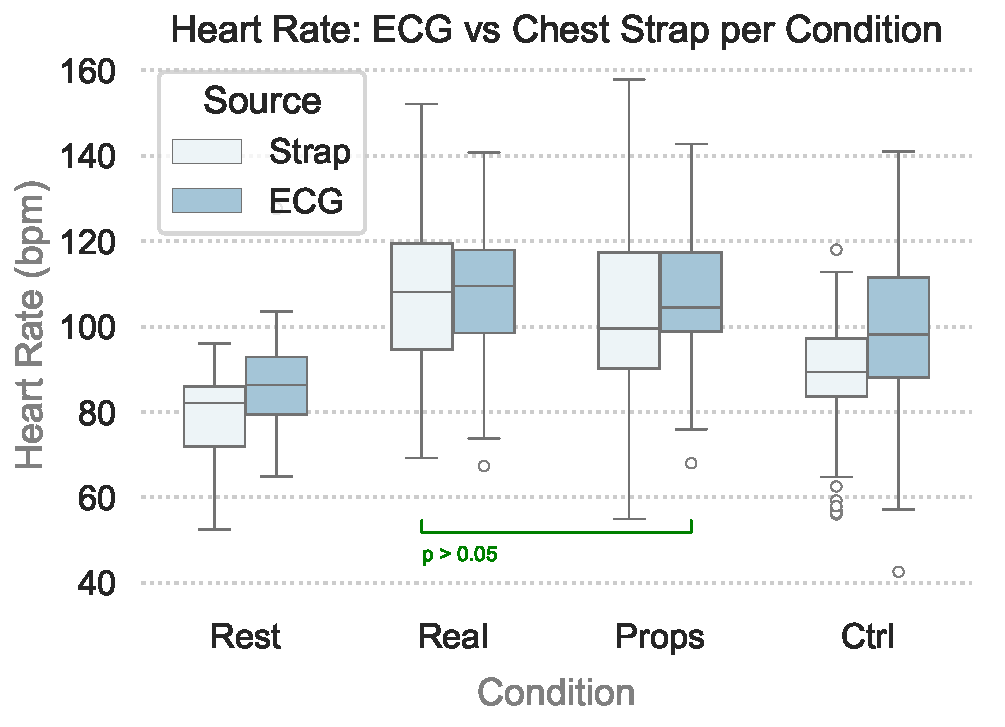
\includegraphics[width=\textwidth]{include/images/hr_per_condition_by_source.pdf}
		\caption{Average \glsfirst{HR} measured before (0) and during the conditions (A, B, and C) using \gls{ECG} and a chest strap}
		\label{fig:physical-exertion-hr}
	\end{subfigure}
	\hspace*{\fill}
	\begin{subfigure}[t]{0.49\columnwidth}
		\centering
		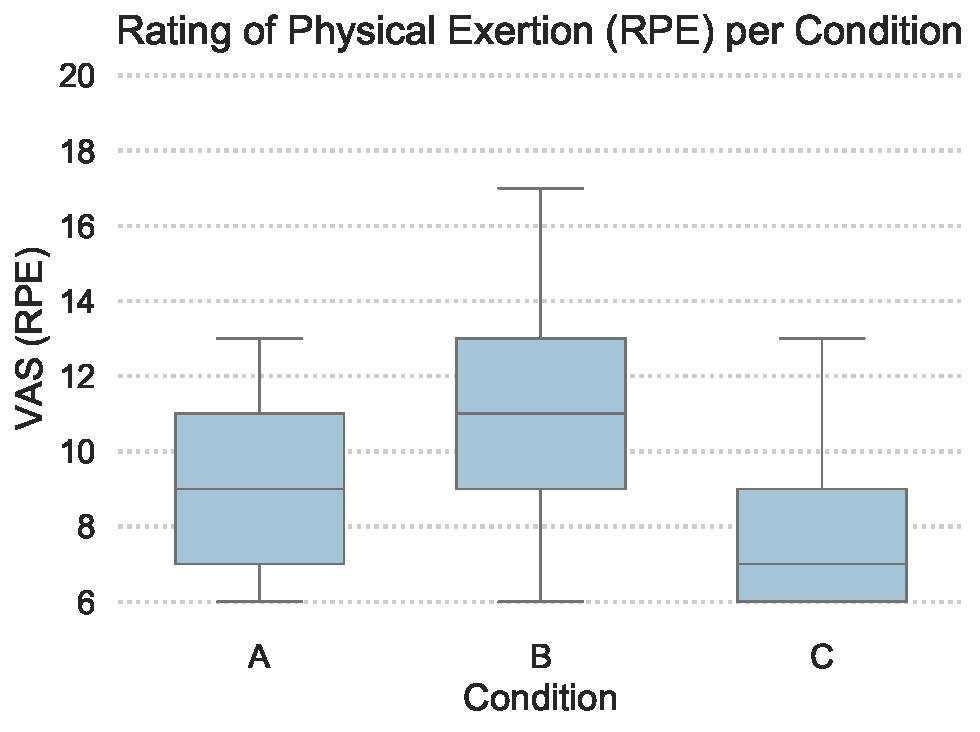
\includegraphics[width=\textwidth]{include/images/rpe_per_condition.pdf}
		\caption{Average \glsfirst{RPE} as reported via \glsfirst{VAS} after each condition (A, B, and C) on a scale from 6 to 20}
		\label{fig:physical-exertion-rpe}
	\end{subfigure}
	\captionsetup{subrefformat=parens}
	\caption[Results: physical exertion]{Results for physical exertion, measured with \gls{HR} on the one hand \subref{fig:physical-exertion-hr}, and by self report \subref{fig:physical-exertion-rpe} on the other}
	\label{fig:physical-exertion}
\end{figure}